\chapter{Evolutionary Computation}
\label{chap:evo}

\section{Evolutionary Algorithms}

Evolutionary Algorithms, and more globally Evolutionary Computation, are bio-inspired approaches based on the idea of using some mechanisms of biological evolution \cite{origin-of-species} and genetics \cite{genetics} in computational methods \cite{introduction-ga}. 

Evolutionary algorithms are stochastic optimization methods that use a population of candidate solutions (or \textit{individuals}) to iteratively reach an optimal or quasi-optimal solution by selecting the fittest individuals at each generation. They can use mutation operators, which modify some characteristics of an individual, and crossover operators that create children sharing traits with 2 (or more) parents from the population, in a process described in figure \ref{fig:GA}.

Evolutionary Algorithms can be characterized at different levels, as seen in figure \ref{fig:GP-classes}:
\begin{itemize}
    \item \textbf{Gene}: Based on biological genetics, genes are the basic blocks of the individual, each defining a parameter such as the value of an argument or a simple rule.
    \item \textbf{Genome}: This group of genes describes an individual 
    \item \textbf{Phenotype}: Once expressed, the genome creates the phenotype, for example a graph from a list of genes each defining the weight of a link between 2 nodes.
    \item \textbf{Problem}: Some algorithms can solve static problems like the Rastrigin function while others optimize policies, for example investment strategies.
    \item \textbf{Fitness function}: The fitness function evaluates how well the individual is adapted to the problem, e.g. by computing the mean error or any function designed to be maximized by the algorithm.
\end{itemize}


\begin{figure}[H]
 \centering
 \captionsetup{justification=centering, margin=0.5cm}
 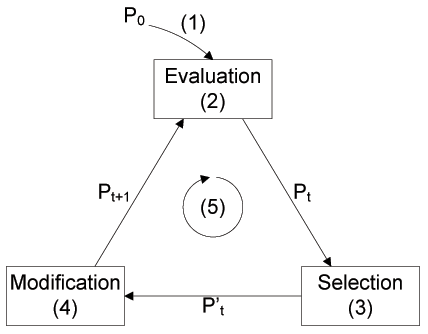
\includegraphics[width=9cm]{images/GA.png}
 \caption{Illustration of the steps of an Evolutionary Algorithm.}
\small\textsuperscript{Dennis Wilson, \url{https://github.com/d9w/evolution/blob/master/2_ga/1_GAs.ipynb}}
 \label{fig:GA}
\end{figure}

Evolutionary algorithms follow the same steps, as illustrated in figure \ref{fig:GA}: (1) A population $P_0$ of random individuals is created, (2) At each generation $t$, each individual in population $P_t$ is evaluated and assigned a fitness value based on the evaluation, (3) Some individuals are selected based on their fitness, (4) Mutation and Crossover operators create new individuals and generate the population $P_{t+1}$ for generation $t+1$, (5) This iteration is repeated until a stopping criterion (e.g. performance, computation cost) is reached.
\\


The defining components of an evolutionary algorithm are the design of a \textit{genetic encoding} which encodes an individual into genes, the \textit{genotype-to-phenotype mapping} which creates an individual from its genes, the  \textit{evolutionary operators} of mutation and crossover than create new individuals, and the \textit{population selection} method to conserve the best traits.

% DGW: Move caption text here as a paragraph referring to figure 2.1. Captions should be used only to describe the image. 
% Add something like: The design of a genetic encoding, the genotype-to-phenotype mapping,  the evolutionary operators of crossover and mutation, and the population selection method are the defining components of an evolutionary algorithm.

\begin{figure}[H]
 \centering
 \captionsetup{justification=centering, margin=0.5cm}
 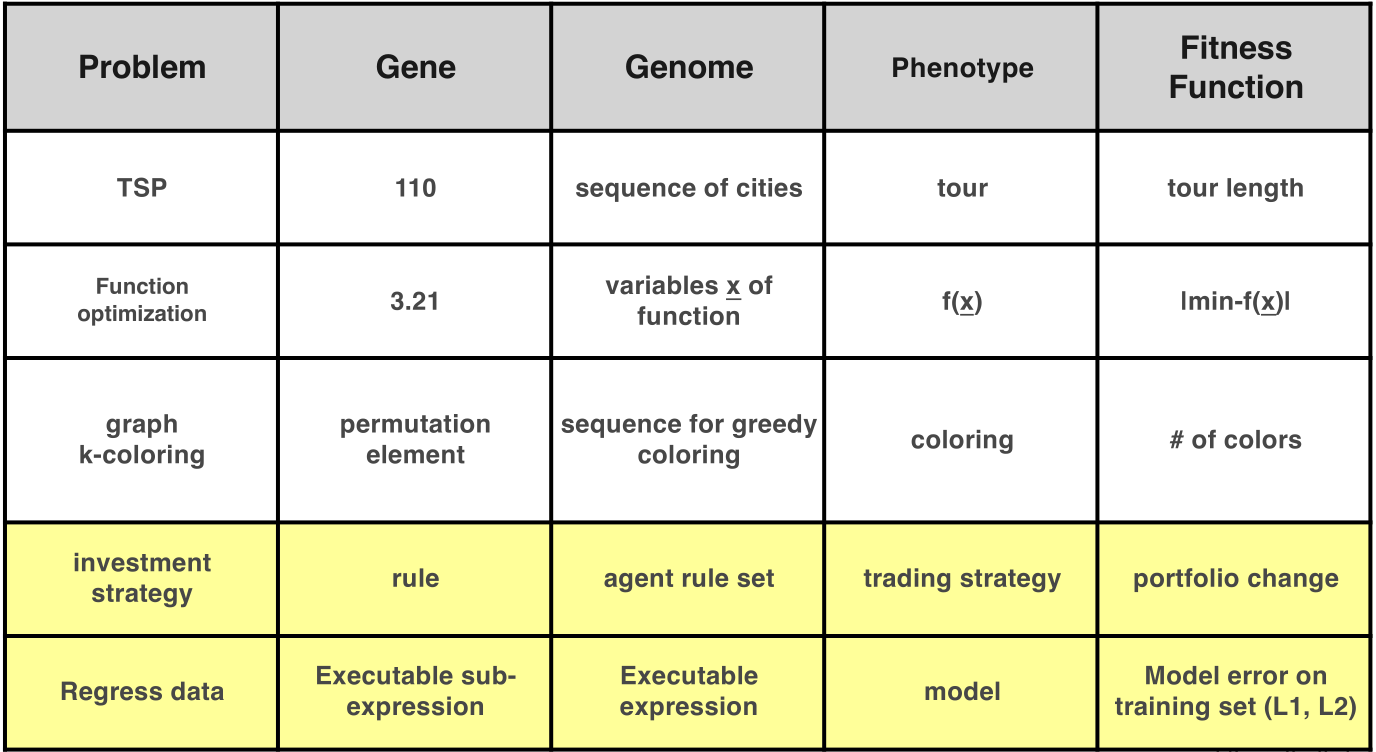
\includegraphics[width=14cm]{images/gp_types_of_eas.png}
 \caption{\label{fig:GP-classes} Evolutionary Algorithms: examples of problems and individual encodings. Examples in white are static problems which can use a direct problem encoding in the genome. Examples in yellow show the evolution of a policy or function. \cite{intro-gp}}
\end{figure}

\section{Evolution of policies}

While Genetic Algorithms are optimization algorithms, Evolutionary Programming evolves functions or policies in an environment they interact with. It relies on the same mechanisms as Evolutionary Algorithms, except the individuals are functions. Mutation and crossover operators are defined on these functions, and selection is based on the behavior of each individual through the total reward they collect during a run. This total reward can then be adjusted to compute the fitness by favoring diverse behaviors or phenotypes. By optimizing for the most efficient behavior, these algorithms look for the function that solved the problem best. 
% DGW: describe how this creates fitness or selection in a GA
These functions can be for example defined as graphs like Cartesian Genetic Programming \cite{CGP}, or as neural networks like NEAT \cite{NEAT_1}.

In addition to previously shown features, individuals in Evolutionary Programming algorithms can be characterized by their behavior in an environment. We can hence look at \textbf{Genotype}, \textbf{Phenotype}, and \textbf{Behavior} for a mapping of individuals in a problem. Even though individuals may share similar genotypes or phenotypes, their behaviors may differ due to the impact of the environment. 

Optimizing functions to be used as policies through evolutionary algorithms is the field of Evolutionary Reinforcement Learning, as described in section \ref{sec:ERL}.

\section{NeuroEvolution}

Neuroevolution is the field which tries to evolve neural network, i.e. their weights and/or architecture, through evolutionary algorithms. Two main approaches have arisen to tackle this issue: directly encoding the network, and using a generator to create it indirectly.

\subsection{Direct encoding of an ANN}
The first approach relies on directly encoding the final neural network, used to choose an action during the game, as an individual for the genetic algorithm. Each weight is therefore directly mutated by the algorithm.

\subsubsection{Weight Evolution with Evolution Strategies}
Similarly to a gradient-based methods, this technique aims to optimize synaptic weights and biases in a neural network by using evolutionary algorithms such as Covariance Matrix Adaptation Evolution Strategy (CMA-ES) \cite{CMA-ES} \cite{CMAES-Atari}.

CMA-ES is a population-based stochastic derivative-free method that creates new populations based on a distribution, which evolves from the distribution in the previous generation based on which candidates performed best (Fig. \ref{CMA-ES}).

\begin{figure}[H]
 \centering
 \captionsetup{justification=centering, margin=0.5cm}
 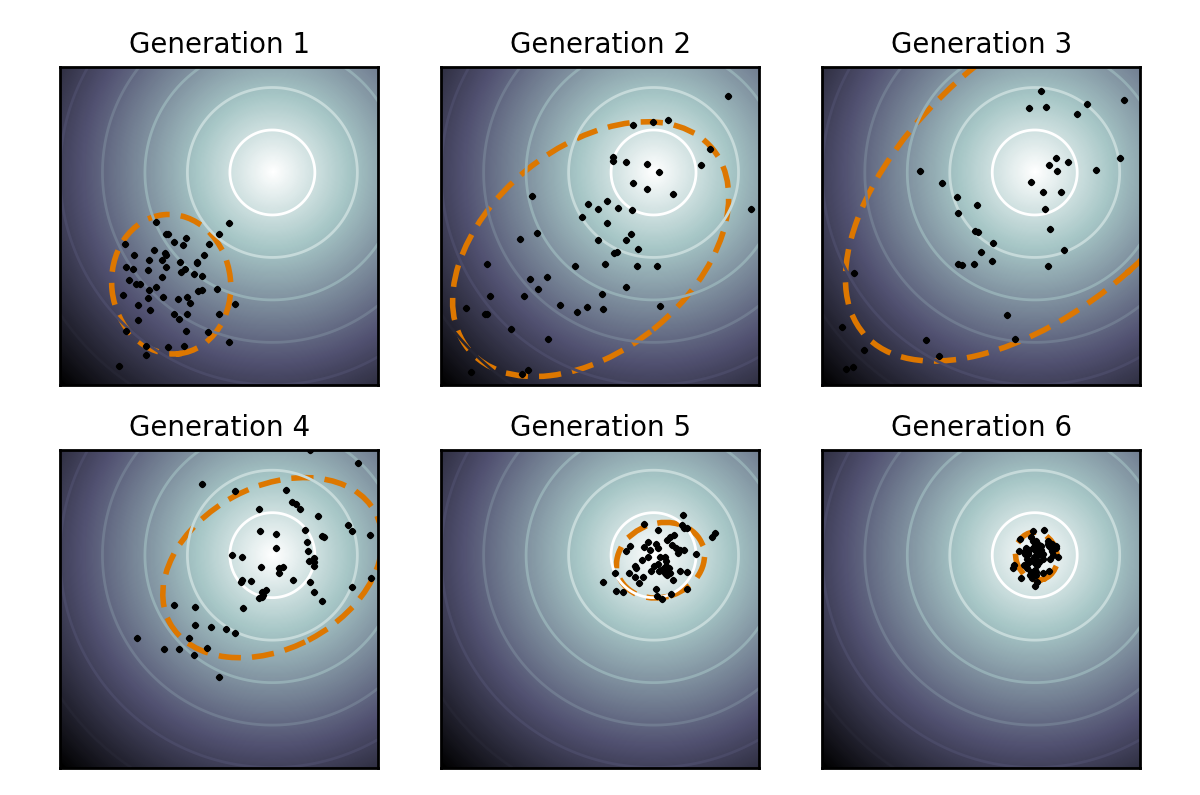
\includegraphics[width=7cm]{images/CMA_ES.png}
 \caption{\label{CMA-ES}Illustration of an actual optimization run with CMA-ES on a simple two-dimensional problem. The spherical optimization landscape is depicted with solid lines of equal-values. The population (dots) is much larger than necessary, but clearly shows how the distribution of the population (dotted line) changes during the optimization. \cite{wiki:cmaes}}
 \label{CMA-ES}
\end{figure}
%DGW: prefer citing Wiki (https://en.wikipedia.org/wiki/Wikipedia:Citing_Wikipedia)

\bigbreak

\subsubsection{NeuroEvolution of Augmenting Topologies}
% DGW: In section titles, prefer full names over acronyms

% DGW: definition of ANN architecture should be previously defined / DONE
Since the architecture of a neural network (e.g. number of layers, size of each layer, recurrent units) can have a strong impact on final performance, this technique evolves simultaneously both network structure and neuron weights of the final network. The NeuroEvolution of Augmenting Topologies (NEAT) algorithm created in 2002 (\cite{NEAT_1, NEAT_2}) presents solutions to 3 fundamental issues in the evolution of neural networks:
%DGW: NEAT_1 and NEAT_2 Bibtex entries are wrong / DONE



\begin{itemize}
    \item \textbf{Crossover between different structures}: NEAT provides a genotype-to-phenotype mapping based on mutations (Fig. \ref{NEAT}).
    \item \textbf{Protection of topological innovation}: The speciation mechanism evaluates candidates by comparing them to similar architectures to allow new structures to mature without being instantly eliminated. 
    \item \textbf{Minimization of structural complexity}: Nodes are added to a minimal initial structure in order to prevent networks from being too big without benefits.
\end{itemize}
\bigbreak

% DGW: specify how NEAT is a direct encoding method

Since NEAT directly uses the network it evolves as the policy, it is a direct encoding method: the phenotype is built from the genotype in one step.

Multiple variants have been created from NEAT, including rtNEAT \cite{rtNEAT} for real-time neuroevolution, FS-NEAT \cite{FS-NEAT} for feature selection, or HyperNeat based on indirect encoding \cite{HyperNEAT}.

\begin{figure}[H]
 \centering
 \captionsetup{justification=centering, margin=0.5cm}
 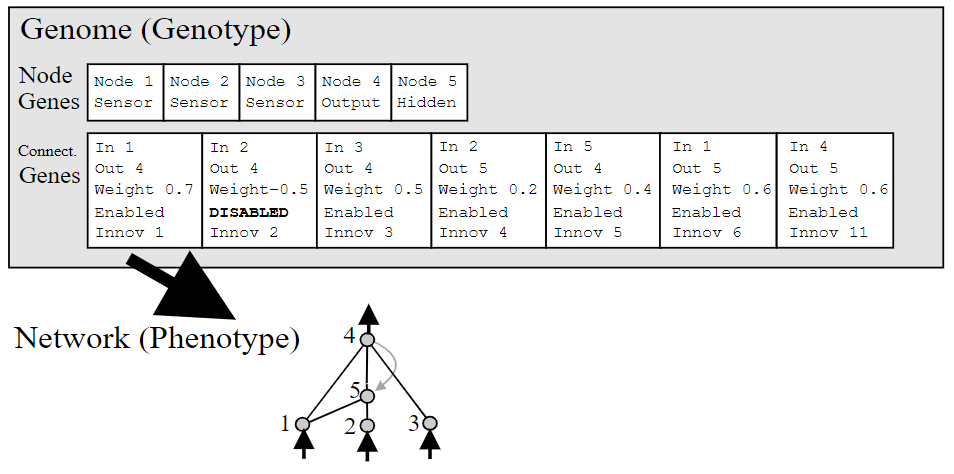
\includegraphics[width=14cm]{images/neat.png}
 \caption{\label{NEAT}NEAT genotype-to-phenotype mapping example. A genotype is depicted that produces the shown phenotype. There are 3 input nodes, one hidden, and one output node, and seven connection definitions, one of which is recurrent. \cite{NEAT_2}}
 \label{fig:NEAT}
\end{figure}

Further details on NEAT are given in \ref{chap:neuroevo}.

\subsection{Indirect encoding of Neural Networks}
%DGW section titles should make sense independently when possible

The second approach uses an intermediary program, optimized through an evolutionary algorithm, to generate the synaptic weights of the final neural network based on their positions. This method reduces the search space to a more efficient one by reusing the same information multiple times, since the same program is used for each and every connection across the final network. 

%DGW: what is a CPPN?
HyperNEAT \cite{HyperNEAT} uses a Compositional Pattern Producing Network (CPPN) \cite{CPPN} optimized by a NEAT-based process to create the final network. CPPNs are Artificial Neural Networks that implement multiple activation functions including Gaussian, sigmoid, and periodic functions such as sine or cosine, adding symmetry patterns to their outputs relative to their inputs.

Using a CPPN as intermediate network allows the final network to be larger without increasing the size of the space to explore, since the same CPPN can be used on any number of neurons. The symmetry patterns of the CPPN also produce connectivity patterns in the final network based on the positions of the neurons, better exploiting regularities in the task.

\section{Quality Diversity approaches}

While most evolutionary approaches focus on directly finding the individual with the highest fitness, the family of Quality-Diversity algorithms \cite{quality-diversity} favors solutions both diverse and high-performing. Since some RL problems can be very deceptive for neuroevolution (cf figure \ref{fig:maze}), evolving more varied behaviors can lead to better-performing solutions and avoids getting stuck in dead-ends.

\begin{figure}[H]
 \centering
 \captionsetup{justification=centering, margin=0.5cm}
 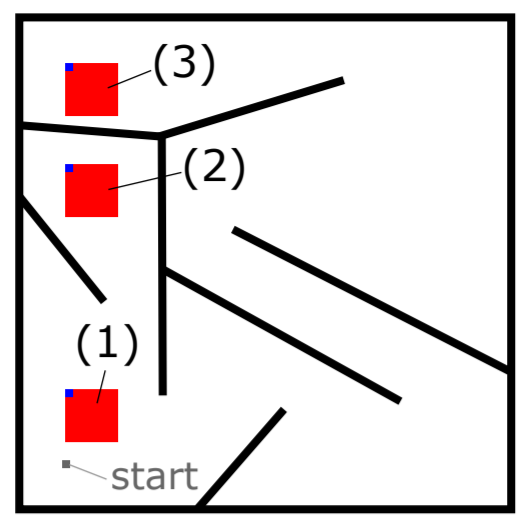
\includegraphics[width=5cm]{images/deceptive-maze.PNG}
 \caption{\label: Deceptive maze in which (1) is the start region,
(2) is the dead-end region, and (3) is the exit region. Evolution based on distance to the exit region leads to individuals being stuck in the dead-end region. \cite{novelty-search-theory}}
 \label{fig:maze}
\end{figure}

\subsection{Novelty search}

Novelty Search \cite{novelty-only} replaces the fitness function in a problem with a \textit{novelty score}, which defines how novel the behavior of the individual is compared to previously encountered populations. It hence pushes towards more diversity, to cover the search space: it is a \textit{divergent} evolution technique.

Novelty Search with local competition \cite{novelty-search-local-competition} applies this principle while still using the fitness score to keep the best-performing individuals in each niche, without inducing competition between individuals of different niches.

\begin{figure}[H]
 \centering
 \captionsetup{justification=centering, margin=0.5cm}
 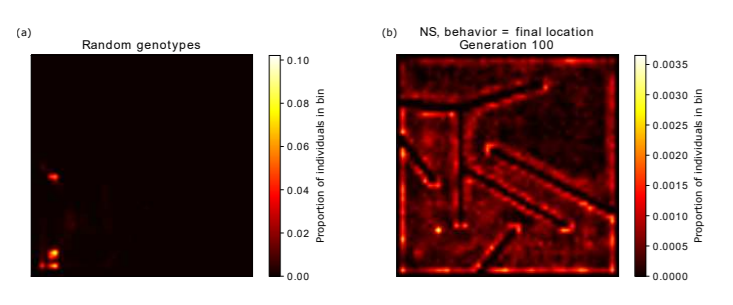
\includegraphics[height=6cm]{images/novelty-maze.PNG}
 \caption{\label: Solutions generated by (a) a random search of 10000 individuals in the genotype space and by (b) 100 generations of 100 individuals via novelty search. \cite{novelty-search-theory}}
 \label{fig:Map-elites}
\end{figure}

\subsection{MAP-Elites}
% DGW: what is an elite ?
In population-based algorithms like Evolutionary programming, elites are the best elements in a population, or in a local sub-population. Keeping the elites from a generation to the next in order to be sure to not lose the best individuals is called \textit{elitism}.

The  Multi-dimensional Archive of
Phenotypic Elites (\textit{MAP-Elites}) algorithm \cite{MapElites} aims at \textit{illuminating the search space}, i.e. exploring the search space and keeping local elites in a discretized map of the space. By characterizing behavior with features independent from the fitness, MAP-Elites discovers diverse behaviors, and can show the fitness landscape of the problem and how attributes of solutions contribute to performance. 

\begin{figure}[H]
 \centering
 \captionsetup{justification=centering, margin=0.5cm}
 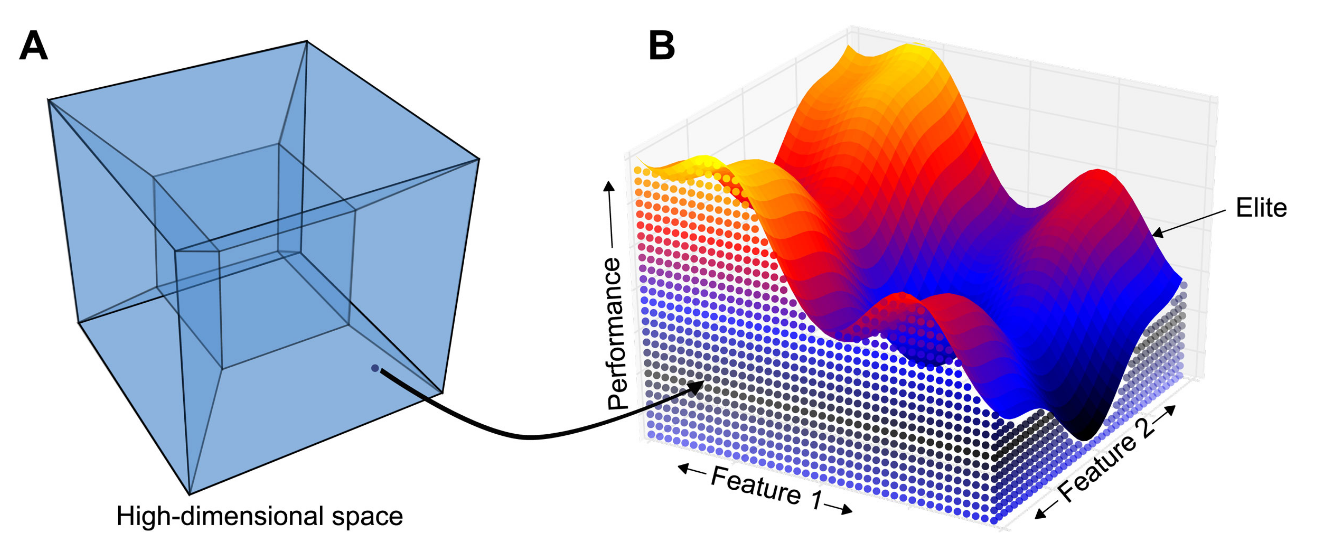
\includegraphics[height=6cm]{images/illumination.png}
 \caption{\label: The MAP-Elites algorithm searches in a high-dimensional space to find the highest-performing solution at each point in a low-dimensional feature space, where the user gets to choose dimensions of variation of interest that define the low dimensional space. \cite{MapElites}}
 \label{fig:Map-elites}
\end{figure}

%%% mode: latex
%%% TeX-master: "isae-report-template"
%%% End: 
